
\section{Motivation}

Qi  Go girl go !


\section{Methodology}
The concept of "livability" lacks clearly defined theoretical framework in the literature \citep{giap2014new}. This complex measure is often used in empirical studies, to rank and compare different geographical areas in terms of the "quality of life" or "well-being" offered to their inhabitants. The last three decades of research on happiness has shown that the well-being should be measured with social, economical and also subjective to the given group set of indicators \citep{diener1997measuring}. In cities, livability is often defined in terms of greenery, security, economic stability, infrastructure and night life \citep{ unit2011liveanomics}.  
Number of city rankings have been published by institutions such as C40, the World Economic Forum \citep{Okulicz-Kozaryn2013}. However, for the purpose of this study, each of the existing methodologies required its adaptation to the city district level.  

\subsection{Liveability Standards in Cities}

The "Methodology for Collection and Computation of Liveability Standards in Cities" developed by Government of India breaks down the Index calculation 
to its primary components \citep{methodology}.
The methodology divides the liveability standards indicators in the cities into four pillars: 1. Institutional, 2. Social, 3. Economic and 4. Physical. 
For each pillar "Sub-Indexes" were calculated and weighted respectively with 25\%, 25\%, 5\% and 45\% towards final Index. To calculate the sub-Indexes, respective normalized indicators were added.   

A total of 79 indicators are used for the calculation of the Liveability Index. To eliminate the issue of difference in units and scales, each of the indicators was normalized using the equation \ref{eq:1} (variable has positive impact on the Index) or equation \ref{eq:2}  (negative impact).      
\begin{equation}
I_i^+ = \frac{I_i- I_{min}}{I_{max}- I_{min}}
\label{eq:1}
\end{equation}
 
 \begin{equation}
I_i^- = \frac{I_{max}- I_i}{I_{max}- I_{min}}
\label{eq:2}
\end{equation}

\subsection{Adaptation of the methodology to districts of Berlin}
 
The Berlin Districts Liveability Index adapts the described in the section 1.2.1 methodology for the purpose of district comparison. Taking into account current socio-economic situation and potential measurable differences between districts, the Index is based on four pillars with following the argumentation:
\\ 
\textbf{1. Physical}: Berlin is facing rapid population increase and shortage of housing \citep{Schultheis.2019}. It becomes increasingly difficult to find affordable housing in districts with good infrastructure. Nonetheless, availability of housing is more pressing then the infrastructure. 
\\ 
\textbf{2.Social}: Berlin is well known for night life, which brought more than €1.5 billion to the city in 2018 \citep{Local.2019}. Besides "cool" cultural side, other indicators such as education, health, safety and social support need to be considered. This is the biggest pillar of the index with 16 indicators.
\\
\textbf{3. Economic}: Rapidly growing start-up scene in Berlin and its reputation of being "Silicon Valley of Europe" brings more and more business to the city \citep{cooke2015skill}. Consequently, there is a big competition between districts to attract big players planning to move here (e.g. Google) \citep{Kuhn.2019}. 
\\
\textbf{4. Environmental}: Due to the growing air pollution threat in Berlin \citep{tagesspiegel.2019} and concerns regarding the environmental health in the cities, the Institutional Category of the Index has been replaced by Environmental. The environmental health and greenery of the districts is considered.\\
The methodology for the Berlin District Liveability Index is illustrated by Figure \ref{fig:meth}. Complete list of the indicators and their description can be found in Annex A. 

\begin{figure}[h]

\centering
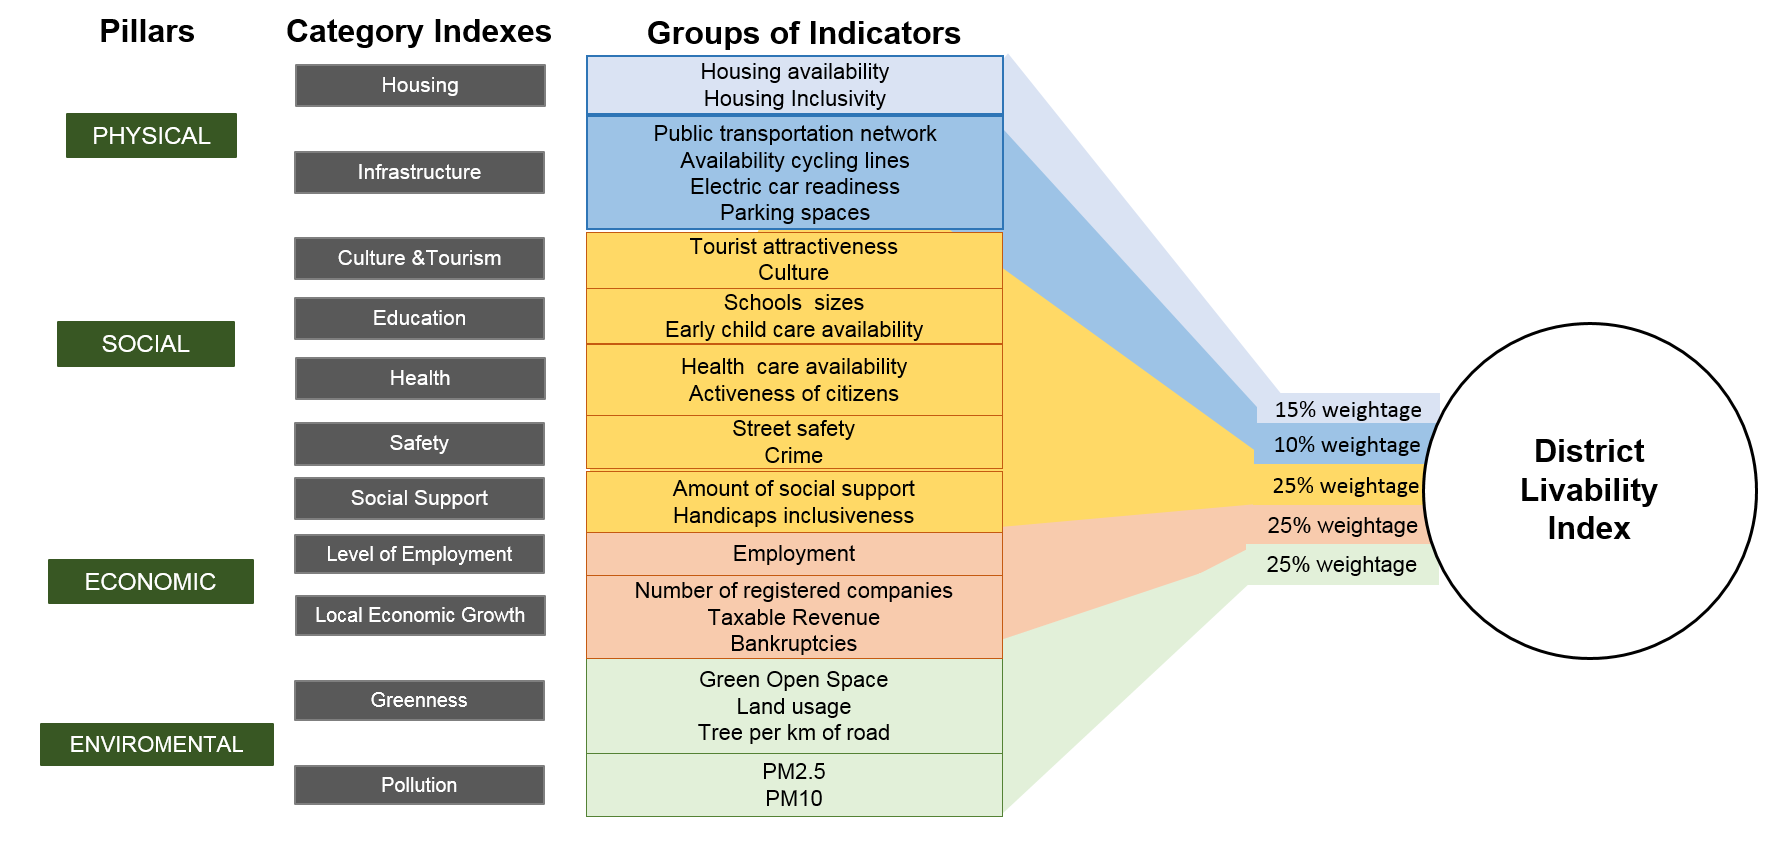
\includegraphics[scale=0.35]{images/Methodology.png}
\caption{Berlin Districts Livability Index Calculation Methodology }
\label{fig:meth}
\end{figure}


